\section{Arc Class Reference}
\label{classArc}\index{Arc@{Arc}}
{\tt \#include $<$arc.h$>$}

Inheritance diagram for Arc::\begin{figure}[H]
\begin{center}
\leavevmode
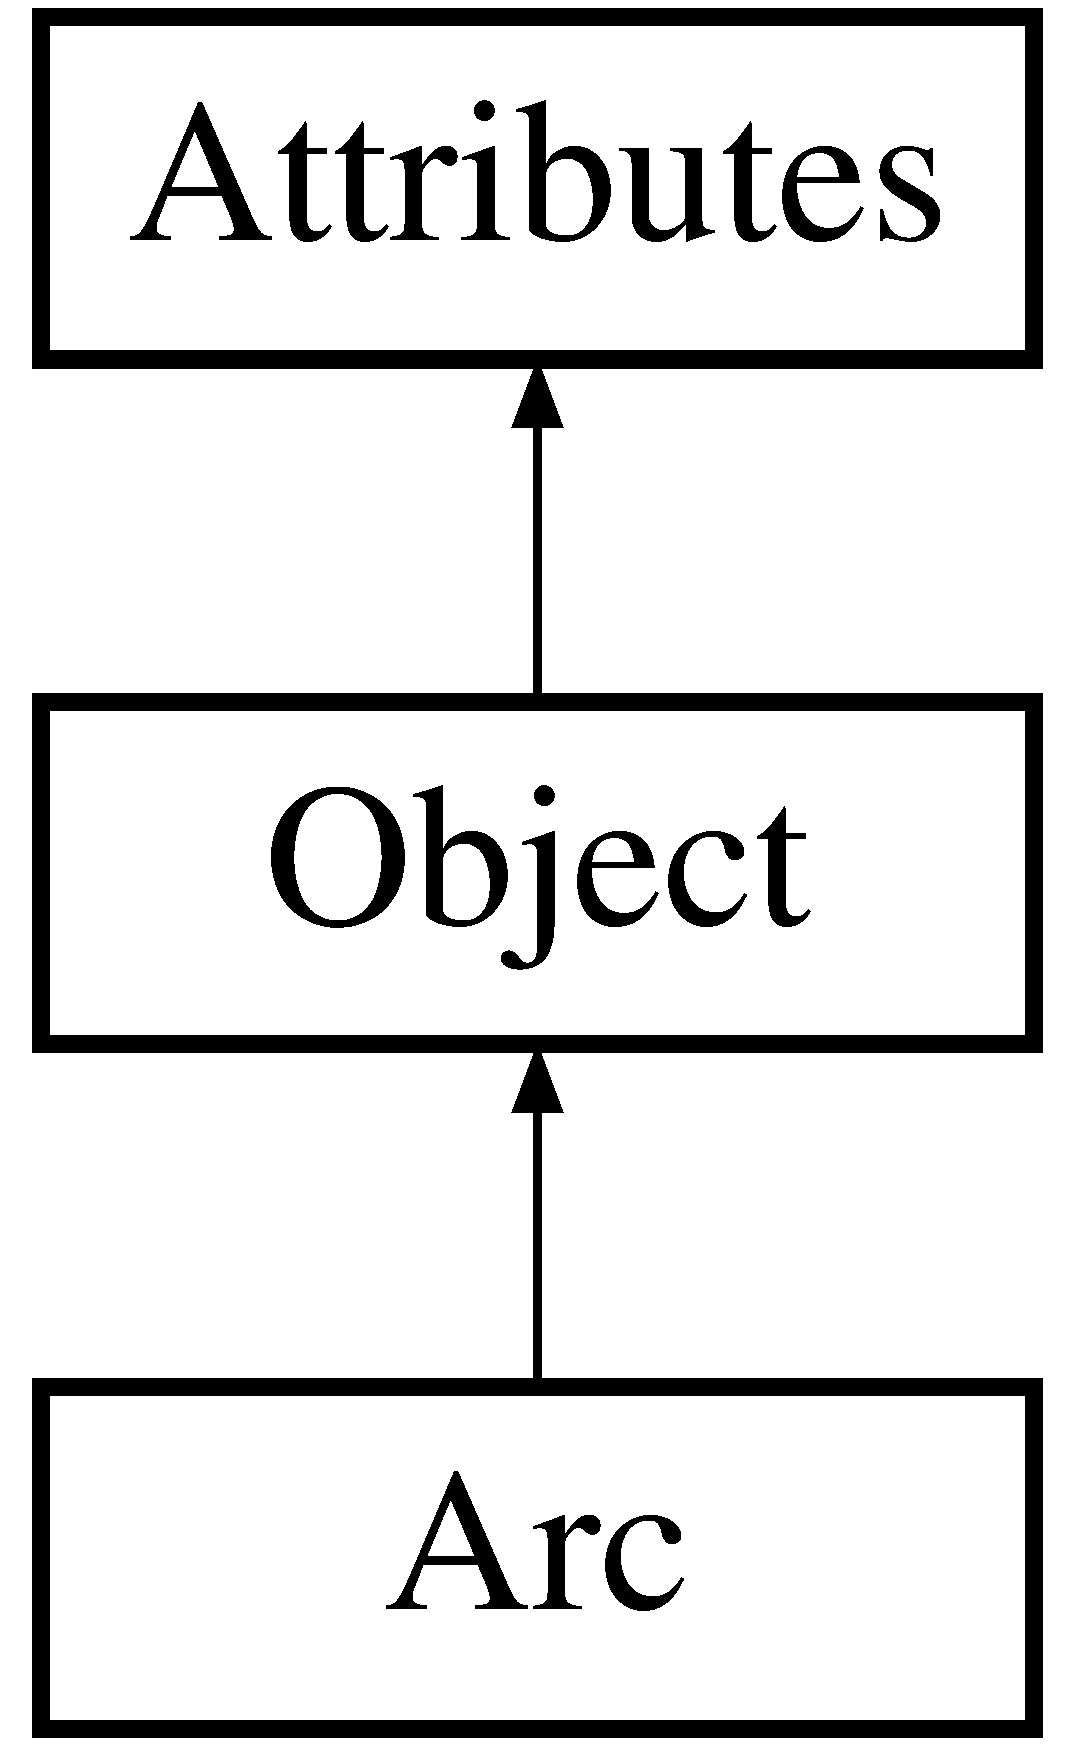
\includegraphics[height=3cm]{classArc}
\end{center}
\end{figure}
\subsection*{Public Types}
\begin{CompactItemize}
\item 
enum {\bf Directions} \{ {\bf Clockwise}, 
{\bf Counter\-Clockwise}
 \}
\item 
enum {\bf Arc\-Types} \{ {\bf Pie\-Wedged} =  0, 
{\bf Open\-Ended} =  1
 \}
\end{CompactItemize}
\subsection*{Public Methods}
\begin{CompactItemize}
\item 
{\bf Arc} ()
\item 
{\bf Arc} ({\bf Coordinate} $\ast$point1, {\bf Coordinate} $\ast$point2, {\bf Coordinate} $\ast$point3)
\item 
{\bf $\sim$Arc} ()
\item 
void {\bf set\-Arc\-Type} ({\bf Arc\-Types} {\bf arc\-Type})
\item 
{\bf Arc\-Types} {\bf get\-Arc\-Type} ()
\item 
{\bf Directions} {\bf get\-Direction} ()
\item 
void {\bf write} (std::ostream \&stream) const
\end{CompactItemize}
\subsection*{Protected Methods}
\begin{CompactItemize}
\item 
void {\bf set\-Direction} ({\bf Directions} {\bf direction})
\item 
double {\bf circum\-Center\-X} ()
\item 
double {\bf circum\-Center\-Y} ()
\item 
{\bf Directions} {\bf clockwise} ()
\item 
double {\bf determinant} (double a1, double a2, double a3, double b1, double b2, double b3, double c1, double c2, double c3)
\end{CompactItemize}
\subsection*{Protected Attributes}
\begin{CompactItemize}
\item 
{\bf Arc\-Types} {\bf arc\-Type}
\item 
{\bf Directions} {\bf direction}
\item 
double {\bf center\-X}
\item 
double {\bf center\-Y}
\item 
{\bf Coordinate} $\ast$ {\bf p1}
\item 
{\bf Coordinate} $\ast$ {\bf p2}
\item 
{\bf Coordinate} $\ast$ {\bf p3}
\end{CompactItemize}


\subsection{Detailed Description}
This class handles arc objects. This class is derived from {\bf Object} {\rm (p.\,\pageref{classObject})}. \begin{Desc}
\item[Author: ]\par
Anthony Liekens \end{Desc}




\subsection{Member Enumeration Documentation}
\index{Arc@{Arc}!ArcTypes@{ArcTypes}}
\index{ArcTypes@{ArcTypes}!Arc@{Arc}}
\subsubsection{\setlength{\rightskip}{0pt plus 5cm}enum Arc::Arc\-Types}\label{classArc_s5}


Enumeration of arc types. The following types can be used to set the type of an arc object : \{$\backslash$tt Pie\-Wedged, Open\-Ended\} \begin{Desc}
\item[Enumeration values: ]\par
\begin{description}
\index{PieWedged@{PieWedged}!Arc@{Arc}}\index{Arc@{Arc}!PieWedged@{PieWedged}}\item[{\em 
{\em Pie\-Wedged}\label{classArc_s5s2}
}]\index{OpenEnded@{OpenEnded}!Arc@{Arc}}\index{Arc@{Arc}!OpenEnded@{OpenEnded}}\item[{\em 
{\em Open\-Ended}\label{classArc_s5s3}
}]\end{description}
\end{Desc}

\index{Arc@{Arc}!Directions@{Directions}}
\index{Directions@{Directions}!Arc@{Arc}}
\subsubsection{\setlength{\rightskip}{0pt plus 5cm}enum Arc::Directions}\label{classArc_s4}


Enumeration of arc directions. The following directions can be used to set the direction of an arc object : \{$\backslash$tt Clockwise, Counter\-Clockwise\} \begin{Desc}
\item[Enumeration values: ]\par
\begin{description}
\index{Clockwise@{Clockwise}!Arc@{Arc}}\index{Arc@{Arc}!Clockwise@{Clockwise}}\item[{\em 
{\em Clockwise}\label{classArc_s4s0}
}]\index{CounterClockwise@{CounterClockwise}!Arc@{Arc}}\index{Arc@{Arc}!CounterClockwise@{CounterClockwise}}\item[{\em 
{\em Counter\-Clockwise}\label{classArc_s4s1}
}]\end{description}
\end{Desc}



\subsection{Constructor \& Destructor Documentation}
\index{Arc@{Arc}!Arc@{Arc}}
\index{Arc@{Arc}!Arc@{Arc}}
\subsubsection{\setlength{\rightskip}{0pt plus 5cm}Arc::Arc ()}\label{classArc_a0}


Constructor. Constructs an arc object. \index{Arc@{Arc}!Arc@{Arc}}
\index{Arc@{Arc}!Arc@{Arc}}
\subsubsection{\setlength{\rightskip}{0pt plus 5cm}Arc::Arc ({\bf Coordinate} $\ast$ {\em point1}, {\bf Coordinate} $\ast$ {\em point2}, {\bf Coordinate} $\ast$ {\em point3})}\label{classArc_a1}


Constructor. Constructs an arc object. An arc is defined by giving three points, a start point, an intermediate point and an end point. These three points lay on the arc. \begin{Desc}
\item[Parameters: ]\par
\begin{description}
\item[{\em 
point1}]First {\bf Coordinate} {\rm (p.\,\pageref{classCoordinate})} defining the arc \item[{\em 
point2}]Second {\bf Coordinate} {\rm (p.\,\pageref{classCoordinate})} defining the arc \item[{\em 
point3}]Third {\bf Coordinate} {\rm (p.\,\pageref{classCoordinate})} defining the arc \end{description}
\end{Desc}
\index{Arc@{Arc}!~Arc@{$\sim$Arc}}
\index{~Arc@{$\sim$Arc}!Arc@{Arc}}
\subsubsection{\setlength{\rightskip}{0pt plus 5cm}Arc::$\sim$Arc ()}\label{classArc_a2}


Destructor. Destructs an arc object. 

\subsection{Member Function Documentation}
\index{Arc@{Arc}!circumCenterX@{circumCenterX}}
\index{circumCenterX@{circumCenterX}!Arc@{Arc}}
\subsubsection{\setlength{\rightskip}{0pt plus 5cm}double Arc::circum\-Center\-X ()\hspace{0.3cm}{\tt  [protected]}}\label{classArc_b1}


Returns the x coordinate of the center of the arc object. \begin{Desc}
\item[Returns: ]\par
double \end{Desc}
\index{Arc@{Arc}!circumCenterY@{circumCenterY}}
\index{circumCenterY@{circumCenterY}!Arc@{Arc}}
\subsubsection{\setlength{\rightskip}{0pt plus 5cm}double Arc::circum\-Center\-Y ()\hspace{0.3cm}{\tt  [protected]}}\label{classArc_b2}


Returns the y coordinate of the center of the arc object. \begin{Desc}
\item[Returns: ]\par
double \end{Desc}
\index{Arc@{Arc}!clockwise@{clockwise}}
\index{clockwise@{clockwise}!Arc@{Arc}}
\subsubsection{\setlength{\rightskip}{0pt plus 5cm}{\bf Arc::Directions} Arc::clockwise ()\hspace{0.3cm}{\tt  [protected]}}\label{classArc_b3}


Calculates the direction of the arc object. \begin{Desc}
\item[Returns: ]\par
{\bf Directions} {\rm (p.\,\pageref{classArc_s4})} \end{Desc}
\index{Arc@{Arc}!determinant@{determinant}}
\index{determinant@{determinant}!Arc@{Arc}}
\subsubsection{\setlength{\rightskip}{0pt plus 5cm}double Arc::determinant (double {\em a1}, double {\em a2}, double {\em a3}, double {\em b1}, double {\em b2}, double {\em b3}, double {\em c1}, double {\em c2}, double {\em c3})\hspace{0.3cm}{\tt  [protected]}}\label{classArc_b4}


Returns the determinant of a 3 by 3 matrix. this function is needed for calculating the circumcenter of an arc, and the direction. \begin{Desc}
\item[Parameters: ]\par
\begin{description}
\item[{\em 
a1}]element on row 1, column 1 \item[{\em 
a2}]element on row 1, column 2 \item[{\em 
a3}]element on row 1, column 3 \item[{\em 
b1}]element on row 2, column 1 \item[{\em 
b2}]element on row 2, column 2 \item[{\em 
b3}]element on row 2, column 3 \item[{\em 
c1}]element on row 3, column 1 \item[{\em 
c2}]element on row 3, column 2 \item[{\em 
c3}]element on row 3, column 3 \end{description}
\end{Desc}
\begin{Desc}
\item[Returns: ]\par
double \end{Desc}
\index{Arc@{Arc}!getArcType@{getArcType}}
\index{getArcType@{getArcType}!Arc@{Arc}}
\subsubsection{\setlength{\rightskip}{0pt plus 5cm}{\bf Arc\-Types} Arc::get\-Arc\-Type ()\hspace{0.3cm}{\tt  [inline]}}\label{classArc_a4}


Returns the type of the arc object. \begin{Desc}
\item[Returns: ]\par
{\bf Arc\-Types} {\rm (p.\,\pageref{classArc_s5})} \end{Desc}
\index{Arc@{Arc}!getDirection@{getDirection}}
\index{getDirection@{getDirection}!Arc@{Arc}}
\subsubsection{\setlength{\rightskip}{0pt plus 5cm}{\bf Directions} Arc::get\-Direction ()\hspace{0.3cm}{\tt  [inline]}}\label{classArc_a5}


Returns the direction of the arc object. \begin{Desc}
\item[Returns: ]\par
{\bf Directions} {\rm (p.\,\pageref{classArc_s4})} \end{Desc}
\index{Arc@{Arc}!setArcType@{setArcType}}
\index{setArcType@{setArcType}!Arc@{Arc}}
\subsubsection{\setlength{\rightskip}{0pt plus 5cm}void Arc::set\-Arc\-Type ({\bf Arc\-Types} {\em arc\-Type})\hspace{0.3cm}{\tt  [inline]}}\label{classArc_a3}


Set the arc type \begin{Desc}
\item[Parameters: ]\par
\begin{description}
\item[{\em 
arc\-Type}]{\bf Arc\-Types} {\rm (p.\,\pageref{classArc_s5})} \end{description}
\end{Desc}
\begin{Desc}
\item[Returns: ]\par
void \end{Desc}
\index{Arc@{Arc}!setDirection@{setDirection}}
\index{setDirection@{setDirection}!Arc@{Arc}}
\subsubsection{\setlength{\rightskip}{0pt plus 5cm}void Arc::set\-Direction ({\bf Directions} {\em direction})\hspace{0.3cm}{\tt  [inline, protected]}}\label{classArc_b0}


Set the arc direction \begin{Desc}
\item[Parameters: ]\par
\begin{description}
\item[{\em 
direction}]{\bf Directions} {\rm (p.\,\pageref{classArc_s4})} \end{description}
\end{Desc}
\begin{Desc}
\item[Returns: ]\par
void \end{Desc}
\index{Arc@{Arc}!write@{write}}
\index{write@{write}!Arc@{Arc}}
\subsubsection{\setlength{\rightskip}{0pt plus 5cm}void Arc::write (std::ostream \& {\em stream}) const\hspace{0.3cm}{\tt  [virtual]}}\label{classArc_a6}


Write the arc object to a given outstream. \begin{Desc}
\item[Parameters: ]\par
\begin{description}
\item[{\em 
stream}]output stream \end{description}
\end{Desc}
\begin{Desc}
\item[Returns: ]\par
void \end{Desc}


Reimplemented from {\bf Object} {\rm (p.\,\pageref{classObject_a3})}.

\subsection{Member Data Documentation}
\index{Arc@{Arc}!arcType@{arcType}}
\index{arcType@{arcType}!Arc@{Arc}}
\subsubsection{\setlength{\rightskip}{0pt plus 5cm}{\bf Arc\-Types} Arc::arc\-Type\hspace{0.3cm}{\tt  [protected]}}\label{classArc_n0}


\index{Arc@{Arc}!centerX@{centerX}}
\index{centerX@{centerX}!Arc@{Arc}}
\subsubsection{\setlength{\rightskip}{0pt plus 5cm}double Arc::center\-X\hspace{0.3cm}{\tt  [protected]}}\label{classArc_n2}


\index{Arc@{Arc}!centerY@{centerY}}
\index{centerY@{centerY}!Arc@{Arc}}
\subsubsection{\setlength{\rightskip}{0pt plus 5cm}double Arc::center\-Y\hspace{0.3cm}{\tt  [protected]}}\label{classArc_n3}


\index{Arc@{Arc}!direction@{direction}}
\index{direction@{direction}!Arc@{Arc}}
\subsubsection{\setlength{\rightskip}{0pt plus 5cm}{\bf Directions} Arc::direction\hspace{0.3cm}{\tt  [protected]}}\label{classArc_n1}


\index{Arc@{Arc}!p1@{p1}}
\index{p1@{p1}!Arc@{Arc}}
\subsubsection{\setlength{\rightskip}{0pt plus 5cm}{\bf Coordinate}$\ast$ Arc::p1\hspace{0.3cm}{\tt  [protected]}}\label{classArc_n4}


\index{Arc@{Arc}!p2@{p2}}
\index{p2@{p2}!Arc@{Arc}}
\subsubsection{\setlength{\rightskip}{0pt plus 5cm}{\bf Coordinate} $\ast$ Arc::p2\hspace{0.3cm}{\tt  [protected]}}\label{classArc_n5}


\index{Arc@{Arc}!p3@{p3}}
\index{p3@{p3}!Arc@{Arc}}
\subsubsection{\setlength{\rightskip}{0pt plus 5cm}{\bf Coordinate} $\ast$ Arc::p3\hspace{0.3cm}{\tt  [protected]}}\label{classArc_n6}




The documentation for this class was generated from the following files:\begin{CompactItemize}
\item 
{\bf arc.h}\item 
{\bf arc.cpp}\end{CompactItemize}
